\chapter{存储体系}
\section{概述}
块管理器BlockManager是Spark存储体系中的核心组件,其初始化在SparkEnv创建过程中,会首先创建BlockManagerMaster,之后再创建BlockManager,最后会在SparkContext中taskscheduler初始化完成后,调用\_env.blockManager.initialize(\_applicationId)完成初始化工作如程序\ref{inputPrg:creatBlockManager}所示
\begin{codeInput}{Scala}{BlockManager的初始化}{creatBlockManager}
//管理所有数据,无论在哪的数据,创建BlockManager
val blockManager = new BlockManager(executorId, rpcEnv, blockManagerMaster,serializer, conf, memoryManager, mapOutputTracker, shuffleManager,blockTransferService, securityManager, numUsableCores)
//blockTransferService的初始化和shuffleClient的初始化,shuffleClient默认是NettyBlockTransferService
blockTransferService.init(this)
shuffleClient.init(appId)
blockManagerId = BlockManagerId(
executorId, blockTransferService.hostName, blockTransferService.port)
//当有外部的ShuffleService时,创建新的BlockManagerId,否则就利用现有的blockManagerId
shuffleServerId = if (externalShuffleServiceEnabled) {
  BlockManagerId(executorId, blockTransferService.hostName, externalShuffleServicePort)
} else {
  blockManagerId
}
//向BlockManagerMaster注册blockManagerId slaveEndpoint
  master.registerBlockManager(blockManagerId, maxMemory, slaveEndpoint)
if (externalShuffleServiceEnabled && !blockManagerId.isDriver) {
  registerWithExternalShuffleServer()
}
\end{codeInput}

程序中在向BlockManagerMaster注册的时候会向判断当前进程是否为Driver。这是因为Driver和Executor中都会对SparkEnv进行初始化,且执行代码相同,

Spark存储体系架构图如\ref{fig:SparkArc}所示
\begin{figure}[H] 
	\centering
	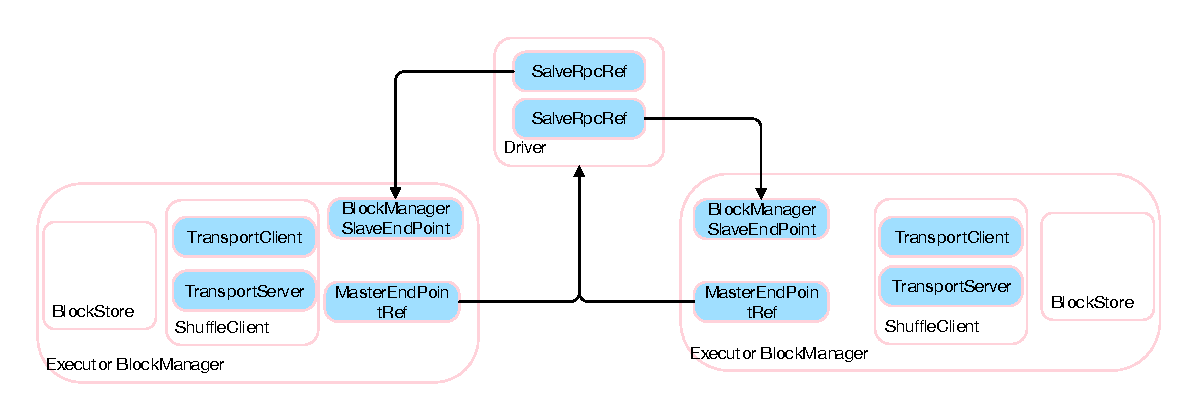
\includegraphics[width=\textwidth]{figures/storage.pdf}
	\caption{Spark存储体系架构}
	\label{fig:SparkArc}
\end{figure}

Spark定义了抽象类BlockStore,用于指定所有的存储类型规范。Spark1.6版本中定义了三种实现MemoryStore、DiskStore和ExternalBlockStore,其类图如图\ref{fig:BlockStore}所示
\begin{figure}[H] 
	\centering
	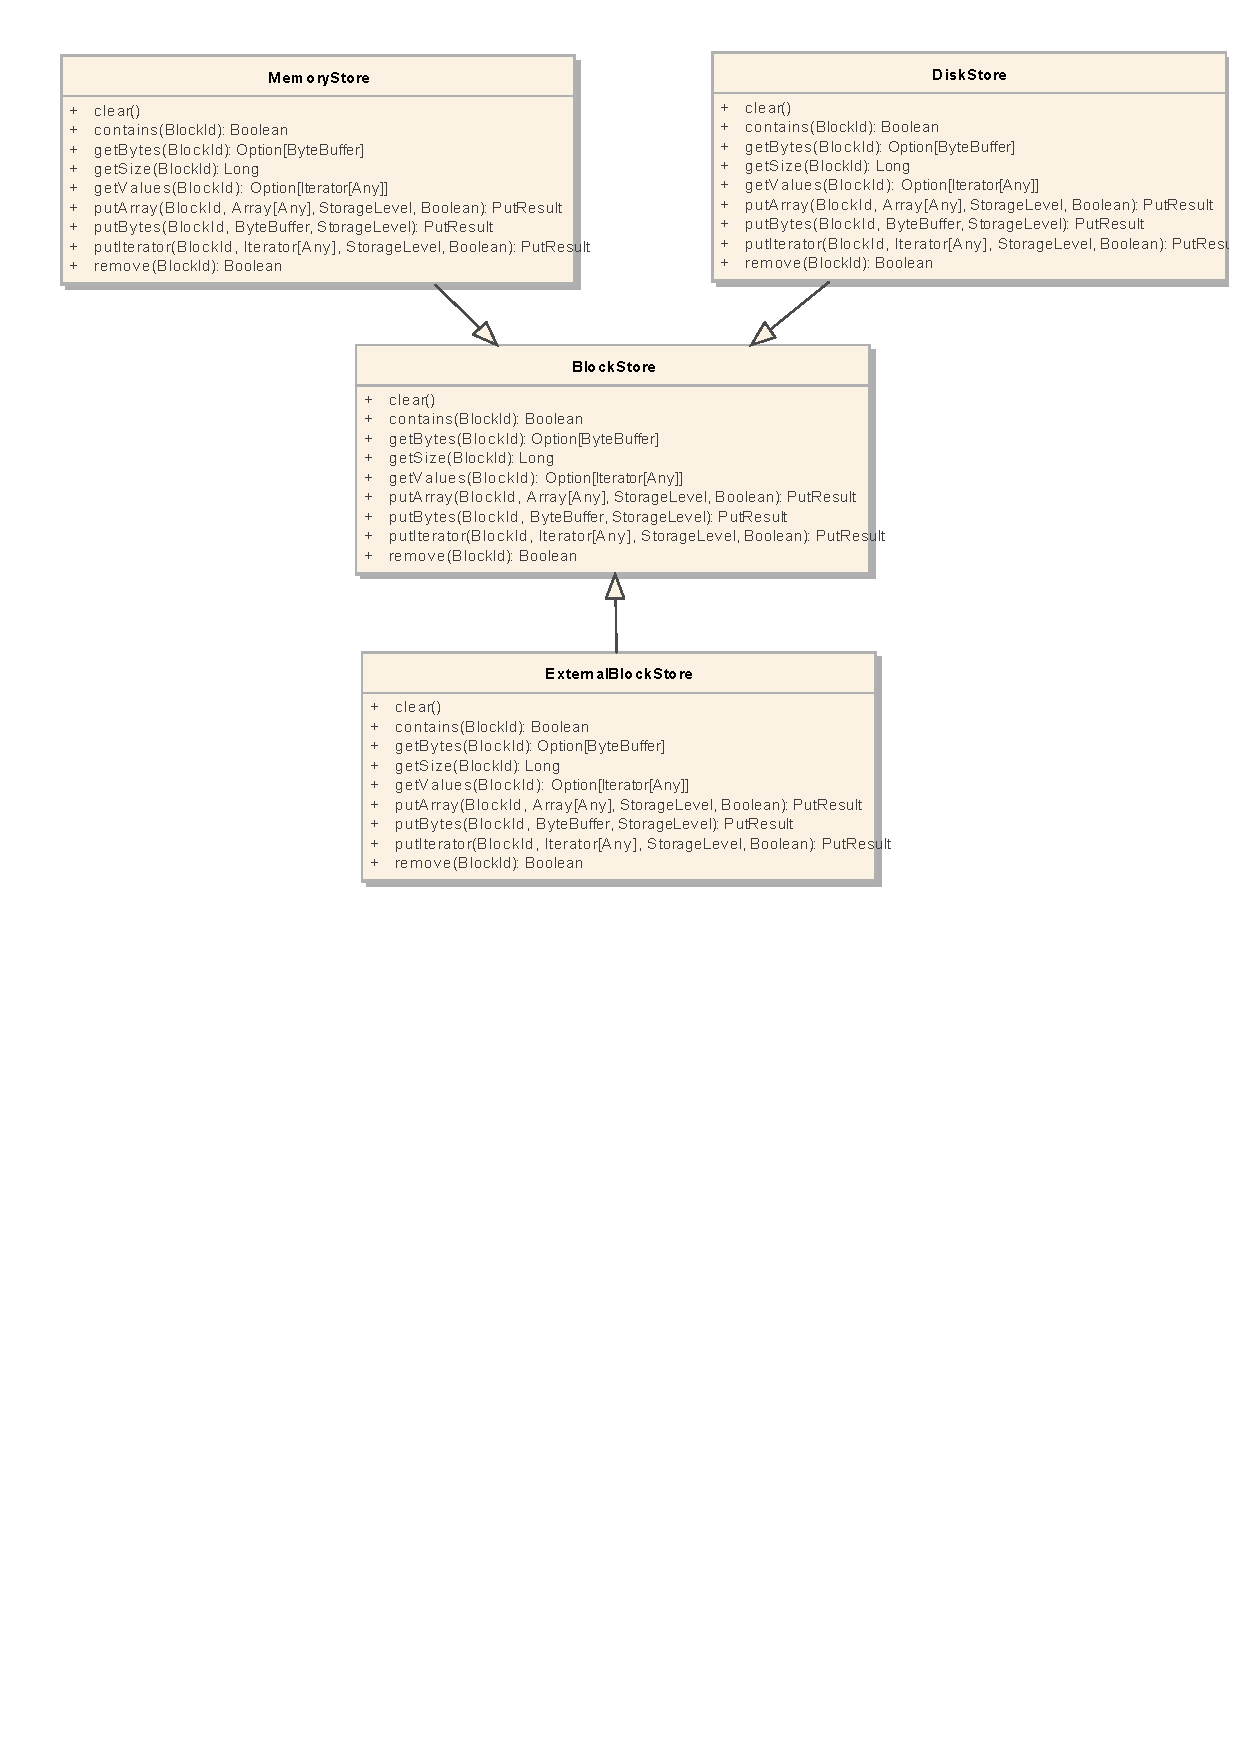
\includegraphics[width=\textwidth]{figures/BlockStore.pdf}
	\caption{BlockStore类图结构}
	\label{fig:BlockStore}
\end{figure}

\section{ShuffleClient模块}
由于Spark是分布式部署的,每个Task最终都运行在不同的机器节点上,map任务的输出结果直接存储在map任务所在的机器的存储体系中,reduce任务极有可能不在同一机器上运行,所以需要远程下载map任务的中间结果,这时存储体系中的ShuffleClient就可以发挥作用了。

ShuffleClient并不只是shuffle的客户端,它即包含了client,可以将shuffle文件上传到其他Executor或者从其他Executor下载文件到本地,同时也为其他Executor提供shuffle服务。在spark1.6中shuffleClient在没有开启externalShuffleService时即为NettyBlockTransferService。其初始化内容如程序\ref{inputPrg:nettyBlockTransferService}所示
\begin{codeInput}{Scala}{nettyBlockTransferService初始化}{nettyBlockTransferService}
override def init(blockDataManager: BlockDataManager): Unit = {
  //创建rpc服务
  val rpcHandler = new NettyBlockRpcServer(conf.getAppId, serializer, blockDataManager)
  var serverBootstrap: Option[TransportServerBootstrap] = None
  var clientBootstrap: Option[TransportClientBootstrap] = None
  if (authEnabled) {
    serverBootstrap = Some(new SaslServerBootstrap(transportConf, securityManager))
    clientBootstrap = Some(new SaslClientBootstrap(transportConf, conf.getAppId, securityManager,
    securityManager.isSaslEncryptionEnabled()))
  }
  //创建TransportContext
  transportContext = new TransportContext(transportConf, rpcHandler)
  //创建RPC客户端工厂
  clientFactory = transportContext.createClientFactory(clientBootstrap.toSeq.asJava)
  //创建Netty服务器TransportServer,端口由spark.blockManager.port控制
  server = createServer(serverBootstrap.toList)
  appId = conf.getAppId
}
\end{codeInput}

\subsection{Block的RPC服务}
在map和reduce两端,当reduce任务需要从远处节点Executor上下载map中间输出时,NettyBlockRpcServer需要提供下载Block文件的功能;同时,为了容错,也需要将Block的数据上传到其他节点,所以NettyBlockRpcServer还提供上传功能。NettyBlockRpcServer核心功能代码如程序\ref{inputPrg:NettyBlockRpcServer}
\begin{codeInput}{Scala}{NettyBlockRpcServer核心实现}{NettyBlockRpcServer}
message match {
  case openBlocks: OpenBlocks =>
    val blocks: Seq[ManagedBuffer]=openBlocks.blockIds.map(BlockId.apply).map(blockManager.getBlockData)
    val streamId = streamManager.registerStream(appId, blocks.iterator.asJava)
    logTrace(s"Registered streamId $streamId with ${blocks.size} buffers")
    responseContext.onSuccess(new StreamHandle(streamId, blocks.size).toByteBuffer)
  case uploadBlock: UploadBlock =>
    val level: StorageLevel =serializer.newInstance().deserialize(ByteBuffer.wrap(uploadBlock.metadata))
    val data = new NioManagedBuffer(ByteBuffer.wrap(uploadBlock.blockData))
    blockManager.putBlockData(BlockId(uploadBlock.blockId), data, level)
    responseContext.onSuccess(ByteBuffer.allocate(0))
\end{codeInput}
\subsection{传输上下文TransportContext}
TransportContext用Java编写,TransportContext既可以创建Netty服务,也可以创建Netty客户端。其构造器代码如程序\ref{inputPrg:TransportContext}所示
\begin{codeInput}{Java}{TransportContext构造器}{TransportContext}
public TransportContext(
TransportConf conf,
RpcHandler rpcHandler,
boolean closeIdleConnections) {
  //主要控制Netty框架提供的shuffle的I/O交互的客户端和服务器线程数量
  this.conf = conf;
  //负责shuffle的I/O服务端在接收到客户端RPC请求后,提供打开Block或者上传Block的RPC处理,此处即为NettyBlockRpcServer
  this.rpcHandler = rpcHandler;
  //在shuffle的I/O客户端对消息进行编码
  this.encoder = new MessageEncoder();
  //在shuffle的I/O服务端对客户端传来的ByteBuf进行解析,防止丢包和解析出错
  this.decoder = new MessageDecoder();
  this.closeIdleConnections = closeIdleConnections;
}
\end{codeInput}
\subsection{RPC客户端TransportClientFactory}
TransportClientFactory是创建Netty客户端TransporClient的工厂类,TransportClient用于向Netty服务端发送RPC请求。
TransportClientFactory主要部分如程序\ref{inputPrg:TransportClientFactory}所示
\begin{codeInput}{Java}{TransportClientFactory构造器}{TransportClientFactory}
public TransportClientFactory(
TransportContext context,
List<TransportClientBootstrap> clientBootstraps) {
  this.context = Preconditions.checkNotNull(context);
  this.conf = context.getConf();
  //缓存客户端列表
  this.clientBootstraps = Lists.newArrayList(Preconditions.checkNotNull(clientBootstraps));
  //缓存客户端连接
  this.connectionPool = new ConcurrentHashMap<SocketAddress, ClientPool>();
  //节点之间去数据的连接数,可以使用属性spark.shuffle.io.numConnectionsPerPeer来设置,默认为1
  this.numConnectionsPerPeer = conf.numConnectionsPerPeer();
  this.rand = new Random();	
  IOMode ioMode = IOMode.valueOf(conf.ioMode());
  //客户端channel被创建时使用的类,spark.shuffle.io.mode来配置,默认为NioSocketChannel
  this.socketChannelClass = NettyUtils.getClientChannelClass(ioMode);
  // TODO: Make thread pool name configurable.
  //根据Netty规范,客户端只有Work组,所以此处创建workerGroup,实际上是NioEventLoopGroup
  this.workerGroup = NettyUtils.createEventLoop(ioMode, conf.clientThreads(), "shuffle-client");
  //汇集ByteBuf但对本地线程缓存禁用的分配器
  this.pooledAllocator = NettyUtils.createPooledByteBufAllocator(
  conf.preferDirectBufs(), false /* allowCache */, conf.clientThreads());
}
\end{codeInput}
\subsection{Netty服务器TransportServer}
TransportServer提供了Netty实现的服务器端,用于提供RPC服务,上传、下载等。
\subsection{获取远程shuffle文件}
在上一节中可以看到在获取远程shuffle文件时调用的是shuffleClient.fetchBlocks,实际上是利用NettyBlockTransferService中创建Netty服务。具体的函数实现如程序\ref{inputPrg:shuffleFetchBlocks}所示
\begin{codeInput}{Scala}{获取远端节点上的shuffle文件}{shuffleFetchBlocks}
override def fetchBlocks(
host: String,
port: Int,
execId: String,
blockIds: Array[String],
listener: BlockFetchingListener): Unit = {
    val blockFetchStarter = new RetryingBlockFetcher.BlockFetchStarter {
      override def createAndStart(blockIds: Array[String], listener: BlockFetchingListener) {
        val client = clientFactory.createClient(host, port)
        new OneForOneBlockFetcher(client, appId, execId, blockIds.toArray, listener).start()
      }
    }
    val maxRetries = transportConf.maxIORetries()
    if (maxRetries > 0) {
      new RetryingBlockFetcher(transportConf, blockFetchStarter, blockIds, listener).start()
    } else {
      blockFetchStarter.createAndStart(blockIds, listener)
    }
}
\end{codeInput}
\subsection{上传shuffle文件}
NettyBlockTransferService的上传功能也是利用了NettyBlockTransferService中创建的Netty服务。具体实现如程序\ref{inputPrg:uploadBlock}所示
\begin{codeInput}{Scala}{uploadBlock实现}{uploadBlock}
override def uploadBlock(
hostname: String,
port: Int,
execId: String,
blockId: BlockId,
blockData: ManagedBuffer,
level: StorageLevel): Future[Unit] = {
  val result = Promise[Unit]()
  //创建Netty服务客户端
  val client = clientFactory.createClient(hostname, port)	
  //将Block的存储级别StorageLevel序列化
  val levelBytes = serializer.newInstance().serialize(level).array()
  //将Block中的ByteBuffer转化为数组,便于序列化	
  val nioBuffer = blockData.nioByteBuffer()	
  val array = if (nioBuffer.hasArray) {
    nioBuffer.array()
  } else {
    val data = new Array[Byte](nioBuffer.remaining())
    nioBuffer.get(data)
    data
  }
  //调用Netty客户端的snedRpc方法将字节数组上传,回调RpcResponseCallback
  client.sendRpc(new UploadBlock(appId, execId, blockId.toString, levelBytes, array).toByteBuffer,
    new RpcResponseCallback {
      override def onSuccess(response: ByteBuffer): Unit = {
        result.success((): Unit)
      }
      override def onFailure(e: Throwable): Unit = {
        result.failure(e)
      }
  })
  result.future
}
\end{codeInput}
\section{BlockManagerMaster对BlockManager的管理}
Driver上的BlockManagerMaster对存在于Executor上的BlockManager统一管理,比如Executor注册BlockManger、更新Executor上Block的最新信息。Spark作为分布式处理框架,在管理上是Driver端持有BlockManagerMasterEndpoint,所有的Executor上会有个BlockManagerMasterEndpointRef,所有的Executor与Driver在BlockManger的交互都依赖于它。
\subsection{BlockManagerMasterEndpoint}
BlockManagerMasterEndpoint只存在于Driver上,在Executor启动时会加载和Driver中一样的SparkEnv,这里会完成对Driver中BlockManagerMasterEndpoint的引用。然后通过其给BlockManagerMasterEndpoint发消息,实现与Driver的交互。
BlockManagerMasterEndpoint维护了很多缓存数据结构,重点看下面三个
\begin{enumerate}[\bfseries 1]
	\item blockManagerInfo
	
	其类型为HashMap[BlockManagerId, BlockManagerInfo],缓存所有的BlockManagerId及其BlockManager的信息
	\item blockManagerIdByExecutor
	
	其类型为HashMap[String, BlockManagerId],缓存executorId与其拥有的BlockManagerId之间的映射关系
	\item blockLocations
	
	其类型为JHashMap[BlockId, mutable.HashSet[BlockManagerId]],缓存Block与BlockManagerId直接的映射关系
\end{enumerate}
\subsection{BlockManagerSlaveEndpoint}
在每个Executor上都会运行一个BlockManagerSlaveEndpoint,用来接收Driver中BlockManagerMaster的消息。在Executor对BlockManager初始化时会调用BlockManagerMaster.registerBlockManager来向Dirver中的BlockManagerMaster注册BlockManger的信息,如程序\ref{inputPrg:registerBlockManager}所示
\begin{codeInput}{Scala}{registerBlockManager}{registerBlockManager}
def registerBlockManager(
blockManagerId: BlockManagerId, maxMemSize: Long, slaveEndpoint: RpcEndpointRef): Unit = {
  logInfo("Trying to register BlockManager")
  tell(RegisterBlockManager(blockManagerId, maxMemSize, slaveEndpoint))
  logInfo("Registered BlockManager")
}
\end{codeInput}

由上面的代码可以看出,Executor端会将blockManagerId、最大内存和BlockManagerSlaveEndpoint封装为RegisterBlockManager消息,通过Executor端持有的BlockManagerMasterEndpointRef向Driver端运行的BlockManagerMaster注册。Driver收到Executor注册的消息后会对传来的消息内容进行处理,具体的处理如程序\ref{inputPrg:driverRegisterBlockManager}所示,注册的时候会对blockManagerIdByExecutor和blockManagerInfo两个HashMap进行数据更新,此时Driver中的BlockManagerMaster就拥有了Executor中BlockManager的信息,且持有了对应的BlockManagerSlaveEndpointRef。
\begin{codeInput}{Scala}{Driver注册BlockManager实现}{driverRegisterBlockManager}
private def register(id: BlockManagerId, maxMemSize: Long, slaveEndpoint: RpcEndpointRef) {
  val time = System.currentTimeMillis()
  //确保blockManagerInfo持有消息中的BlockManagerId及其对应信息
  if (!blockManagerInfo.contains(id)) {
    //确保一个Executor只有一个BlockManagerId
    blockManagerIdByExecutor.get(id.executorId) match {
    //旧的BlockManagerId会被移除
      case Some(oldId) =>
        removeExecutor(id.executorId)
      case None =>
    }
  blockManagerIdByExecutor(id.executorId) = id	
  blockManagerInfo(id) = new BlockManagerInfo(id, System.currentTimeMillis(), maxMemSize, slaveEndpoint)
  }
  //最后向listenerBus推送一个SparkListenerBlockManagerAdded消息
  listenerBus.post(SparkListenerBlockManagerAdded(time, id, maxMemSize))
}
\end{codeInput}
\section{磁盘管理器DiskBlockManager}
磁盘管理器的创建在新建BlockManager实例的时候,它将在spark.local.dir中配置的目录下创建二级目录,二级目录的个数由spark.diskStore.subDirectories指定,默认为64.这些目录里面将会保存Block数据,新建二级目录用于对文件进行散列存储,散列存储可以是所有的文件都随机存放,写入或删除文件都很方便,存取速度快,节省时间。另外一个重要的方法就是getFile,程序要获取磁盘上的文件都是通过getFile进行的,其中subDirs是二维数组,用来缓存一级目录和二级目录。这里也使用了Spark磁盘散列文件存储的实现机制。如程序\ref{inputPrg:getFile}所示
\begin{codeInput}{Scala}{getFile的实现}{getFile}
def getFile(filename: String): File = {
  //根据文件名blockId.name计算哈希值
  val hash = Utils.nonNegativeHash(filename)
  //根据哈希值与本地文件一级目录的总数求余数,记为dirId
  val dirId = hash % localDirs.length
  //根据哈希值与本地文件一级目录的总数求商,此商与二级目录的数据在求余数,记为subDirId
  val subDirId = (hash / localDirs.length) % subDirsPerLocalDir	
  //如果dirId/subDirId目录存在,则获取dirId/subDirId目录下的文件
  val subDir = subDirs(dirId).synchronized {
    val old = subDirs(dirId)(subDirId)
    if (old != null) {
      old
    } else {
      //否则新建dirId/subDirId目录
      val newDir = new File(localDirs(dirId), "%02x".format(subDirId))
      if (!newDir.exists() && !newDir.mkdir()) {
        throw new IOException(s"Failed to create local dir in \$newDir.")
      }
      subDirs(dirId)(subDirId) = newDir
      newDir
    }
  }	
  new File(subDir, filename)
}
\end{codeInput}
\section{内存存储MemoryStore}
MemoryStore存储的是没有序列化的Java对象数组或者序列化的ByteBuffer存储到内存中,Spark中MemoryStore的内存模型如图\ref{fig:memoryStore}所示
\begin{figure}[H] 
	\centering
	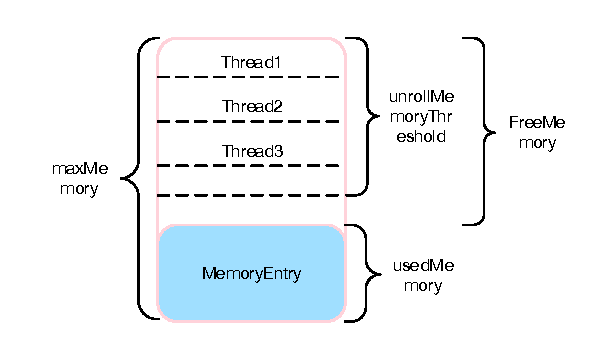
\includegraphics[width=\textwidth]{figures/memoryStore.pdf}
	\caption{MemoryStore的内存模型}
	\label{fig:memoryStore}
\end{figure}

如图\ref{fig:memoryStore}中看出,MemoryStore的存储可以分为两部分
\begin{enumerate}[\bfseries 1]
	\item MemoryEntry组成的usedMemory,这些Memory实际是通过entries持有的
	\item unrollMemoryMap被各线程提前预定,就像占座一样
\end{enumerate}
\section{磁盘存储DiskStore}
当MemoryStore没有足够空间时,就会使用DiskStore将块存入磁盘。